\section{Bayesian Consensus Clustering} \label{bcc-sec-l}

These are only some examples of the different platforms and techniques that are used to measure diverse biological components and are shown in \emph{Fig. \ref{seq-pic}}. 

\begin{figure}[!ht]
\begin{center}
 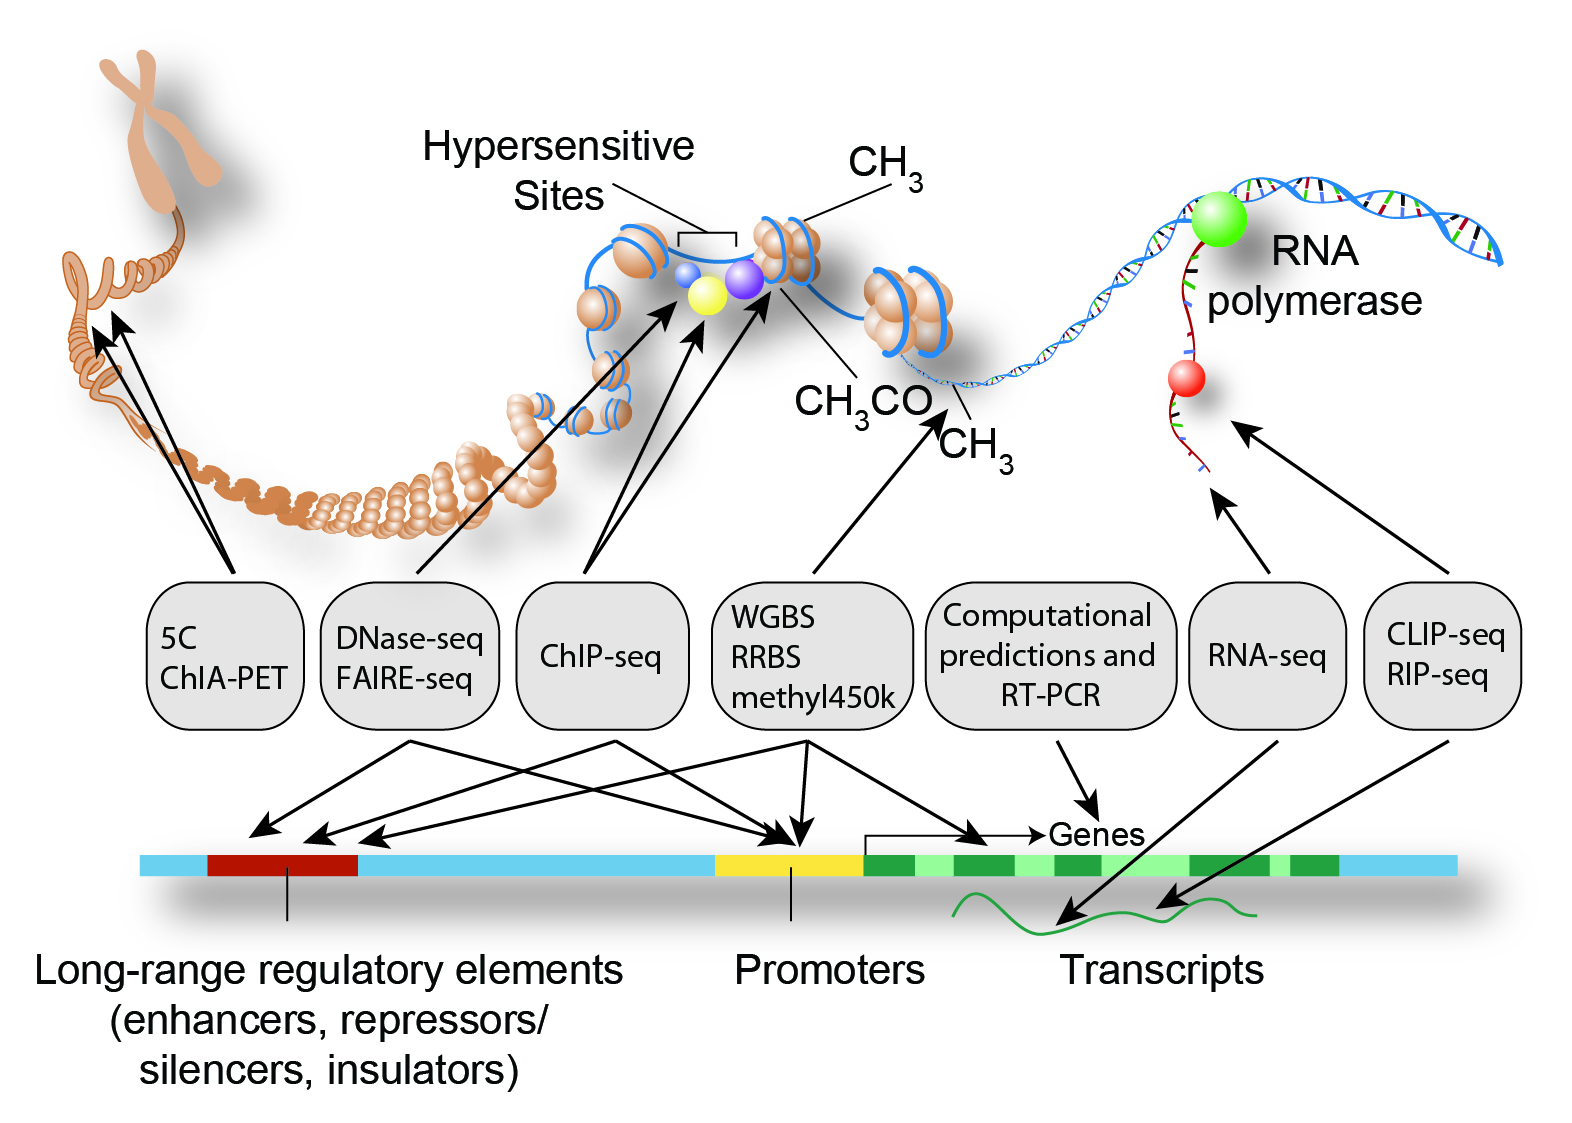
\includegraphics[scale = 0.15]{images/encode-seq.png}
\caption{\emph{Some of the XX-Seq techniques used from the ENCODE projet. Credits: Darryl Leja (NHGRI), Ian Dunham (EBI), Michael Pazin (NHGRI) \citep{Dunham2012}.}}
\label{seq-pic}
\end{center}
\end{figure} 

Bayesian Consensus Clustering can be thought as an extension of a mixture model so as to account for multiple data sources. Thus, before explaining the BCC model the Dirichlet Mixture Model (DMM) will be described, which will put the groundwork in having a better understanding of the integrative model.

The mixture model was described in \emph{Section \ref{cluster-meth-l}}. Under a Bayesian framework the Dirichlet Mixture Model arises, where the parameters themselves are considered as random variables, thus prior distributions will be placed over the random variables. 

If possible, conjugate priors should be used since the posterior distributions will be in the same family as the prior probability distributions. Thus, a natural choice is to use a Dirichlet prior distribution for the mixing proportions $\Pi$. For the parameters $\Theta$, appropriate priors should be chosen depending on the probability distributions that the data follow.

\emph{Figure \ref{fdmm-pic}} shows a graphical representation of the DMM, where $G_{0}$ is the prior probability distribution for the parameters $\theta_{k}$.

% DMM model
\begin{figure}[ht]
  \begin{center}
      % model_pca.tex
%
% Copyright (C) 2012 Jaakko Luttinen
%
% This file may be distributed and/or modified
%
% 1. under the LaTeX Project Public License and/or
% 2. under the GNU General Public License.
%
% See the files LICENSE_LPPL and LICENSE_GPL for more details.

% PCA model

%\beginpgfgraphicnamed{model-pca}
\begin{tikzpicture}

  % Define nodes
  \node[obs]                    (X) {$x_{i}$};
  \node[latent, above=of X] 	(Z) {$z_{i}$};
  \node[latent, above=of Z]  	(p) {$\pi$};
  \node[latent, right=1cm of Z] (t) {$\theta_{k}$};
  \node[latent, above=of t] 	(G) {$G_{0}$};

  % Connect the nodes
  \edge {Z,t} {X} ; %
  \edge {p} {Z} ; %
  \edge {G} {t} ; %

  % Plates
  \plate {} {(t)} {$K$};
  \plate {} {(Z)(X)} {$N$};

\end{tikzpicture}
%\endpgfgraphicnamed

%%% Local Variables: 
%%% mode: tex-pdf
%%% TeX-master: "example"
%%% End: 

  \caption{Graphical representation of the Dirichlet Mixture Model.}
  \label{fdmm-pic}
  \end{center}
\end{figure}

To perform integrative clustering from M different data sources $\mathbb{X}_{1},..., \mathbb{X}_{M}$, the DMM model is extended which leads us to the Bayesian Consensus Clustering (BCC) model \cite{Lock2013}. BCC model assumes that there are N common objects for each data source, where $X_{mn}$ denotes the data for object $n$ from source $m$.
The model is very general and the data sources $\mathbb{X}_{m}$ can have any disparate structure, and each of them requires an arbitrary probability model $f_{m}(X_{mn}|\theta_{m})$.

Let $\mathbb{L}_{m} = (L_{m1},...,L_{mN})$ denote the source specific clusterings and $\mathbb{C} = (C_{1},...,C_{N})$ denote the overall clustering of the data. The model assumes that both $\mathbb{C}$ and $\mathbb{L}_{m}$ will have the same number of possible clusters K, thus $L_{mn} \in \lbrace 1,...,K \rbrace$ and $C_{n} \in \lbrace 1,...,K \rbrace$, will denote the source specific and the overall mixture component for observation $X_{mn}$, respectively.

The source specific clusterings and the overall clustering are related to each other, and the strength of the relation is given by a dependence function $v(L_{mn}, C_{n}, \alpha_{m})$, where $\alpha_{m} \in [\frac{1}{K}, 1]$ is the adherence parameter and controls the adherence of data source $\mathbb{X}_m$ to the overall clustering $\mathbb{C}$. More simply, it explains how much does the source specific clustering for source $m$ agrees with the overall clustering $\mathbb{C}$. So if $\alpha_{m} = 1$, then $\mathbb{L}_{m} = \mathbb{C}$. 

The dependence function $v$ has the form:

\begin{equation}
	v(L_{mn}, C_{n}, \alpha_{m}) = \left\{
	\begin{array}{l l}
		\alpha_{m},\quad \quad \quad if\quad C_{n} = L_{mn}\\
		\frac{1-\alpha_{m}}{K-1},\quad \quad otherwise
	\end{array}\right.
\end{equation}

The graphical representation for the BCC model is given in \emph{Figure \ref{bcc-pic}}, where again $G_{0}$ is the prior for the parameters $\theta_{mk}$.

% BCC model
\begin{figure}[ht]
  \begin{center}
      % model_pca.tex
%
% Copyright (C) 2012 Jaakko Luttinen
%
% This file may be distributed and/or modified
%
% 1. under the LaTeX Project Public License and/or
% 2. under the GNU General Public License.
%
% See the files LICENSE_LPPL and LICENSE_GPL for more details.

% PCA model

%\beginpgfgraphicnamed{model-pca}
\begin{tikzpicture}

  % Define nodes
  \node[obs]                              (X) {$X_{mn}$};
  \node[latent, above=of X] 		(L) {$L_{mn}$};
  \node[latent, above=of L] 		(a) {$\alpha$};
  \node[latent, right=1.4cm of L]  (C) {$C_{n}$};
  \node[latent, above=of C] 		(p) {$\pi$};
  \node[latent, right=1cm of C]  (t) {$\theta_{mk}$};
  \node[latent, above=of t] 		(G) {$\mathcal{G}_{0}$};

  % Connect the nodes
  \edge {L,t} {X} ; %
  \edge {a,C} {L} ; %
  \edge {p} {C} ; %
  \edge {G} {t} ; %

  % Plates
  \plate {} {(t)} {$K$};
  \plate {yx} {(L)(X)} {$M$};
  \plate {} {(C)(X)(yx.north west)(yx.south west)} {$N$};

\end{tikzpicture}
%\endpgfgraphicnamed

%%% Local Variables: 
%%% mode: tex-pdf
%%% TeX-master: "example"
%%% End: 

  \caption{Graphical representation of Bayesian Consensus Clustering.}
  \label{bcc-pic}
  \end{center}
\end{figure}

The full joint distribution of the model by looking at the graphical representation in \emph{Fig \ref{bcc-pic}} is given by:

\begin{equation}\scriptstyle
	P(\mathbb{X}, \mathbb{L}, \mathbb{C}, \Pi , \Theta , \alpha ; \mathcal{H}) = P(\mathbb{X}|\mathbb{L},\Theta) P(\mathbb{L}|\mathbb{C},\alpha) P(\mathbb{C}|\Pi) P(\Pi) P(\alpha) P(\Theta ; \mathcal{H})
\end{equation}

where $\mathcal{H}$ is the set of all the hyper-parameters, related to the parameters $\Theta$. 

To do inference in the Bayesian framework, the posterior distribution of the parameters needs to be computed. By applying the Bayes Rule and conditioning on the observed data $\mathbb{X}$, the posterior distribution is simply proportional to the full joint. Thus:
 
\begin{equation}\scriptstyle
	\begin{aligned}
	& & \scriptstyle P(\mathbb{L},\mathbb{C},\Pi ,\Theta , \alpha | \mathbb{X}; \mathcal{H}) & \scriptstyle \propto P(\mathbb{X}|\mathbb{L}, \mathbb{C},\Pi ,\Theta , \alpha) P(\mathbb{L}, \mathbb{C}, \Pi , \Theta , \alpha; \mathcal{H}) \\
	& & & \scriptstyle = P(\mathbb{X}|\mathbb{L},\Theta) P(\mathbb{L}|\mathbb{C},\alpha) P(\mathbb{C}|\Pi) P(\Pi) P(\alpha) P(\Theta ; \mathcal{H})
	\end{aligned}
\end{equation}

This posterior is intractable to compute, thus we need to resort to approximation schemes and these fall broadly into two classes. Deterministic approximation schemes such as \emph{variational inference} could be used, which are based on analytically approximating the posterior distribution, by assuming that it factorizes in a particular way, or that the posterior will have a specific parametric form, such as a Gaussian, which then we try to approximate.

The other approximation scheme, and the one that is used in this project, is a stochastic approximation of the posterior using Markov Chain Monte Carlo (MCMC) methods. Specifically, \emph{Gibbs sampling} algorithm will be used, which is one of the most popular MCMC algorithms. 

Deriving Gibbs sampling for this model, requires deriving an expression for the \emph{full conditional distribution} of every latent variable conditioned on all the others. Thus, from the graphical model shown in \emph{Figure \ref{bcc-pic}}, we can infer the dependencies of the latent variables by looking at the \emph{Markov blanket} of each variable, which are its neighbours in the graph. 

For mathematical convenience, \emph{conjugate priors} should be used which would allow us to perform analytically some marginalization steps that are necessary in deriving Gibbs sampler. Thus:

\begin{itemize}
	\item $\Pi \sim Dir(\mathbf{\delta_{0}})$. For the mixing proportions a natural choice is a Dirichlet prior distribution, and the hyper-parameter vector $\mathbf{\delta_{0}}$ is set to $(1,...,1)$ so the prior is uniformly distributed in the $K-1$ simplex.
	\item $\alpha_{m} \sim TBeta(\mathit{a_{m}}, \beta_{m}, \frac{1}{K})$. Which means that $a_{m}$ follows a  $Beta$ distribution with parameters $\mathit{a_{m}}, \beta_{m}$ truncated below by $\frac{1}{K}$.
	\item $\theta_{mk} \sim G_{0}$. Where $G_{0}$ is a conjugate prior distribution so that sampling from the conditional posterior $p_{m}(\theta_{mk}|\mathbb{X}_{m}, \mathbb{L}_{m})$ is feasible. For example, if the probability model $f_{m}(X_{mn}|\theta_{m}) \sim Poisson(\lambda_{m})$, then a conjugate prior distribution would be a $Gamma(\lambda_{m}|\mathit{a_{m}}, \beta_{m})$.
\end{itemize}

Having chosen the appropriate prior distributions, the Gibbs sampler would proceed iteratively by sampling from the following full conditional distributions:

\begin{enumerate}
	\item $\scriptstyle \mathbb{L}_{m} | \mathbb{X}_{m}, \Theta_{m}, \mathbb{C}, \alpha_{m} \sim v(L_{mn}, C_{n}, \alpha_{m}) f_{m}(X_{mn}|\theta_{mk}) \quad \text{for} \quad n=1,...,N $
	\item $\scriptstyle \Theta_{m}|\mathbb{L}_{m}, \mathbb{X}_{m} \sim p_{m}(\theta_{mk}|\mathbb{X}_{m}, \mathbb{L}_{m}) \quad \text{for} \quad k=1,...,K $
	\item $\scriptstyle \alpha_{m}|\mathbb{L}_{m}, \mathbb{C} \sim TBeta \big(\mathit{a_{m}}+\sum_{n=1}^{N}\mathbbm{1}(L_{mn}=k,C_{n}=k), \beta_{m}-N-\sum_{n=1}^{N}\mathbbm{1}(L_{mn}=k,C_{n}=k), \frac{1}{K}\big)$
	\item $\scriptstyle \mathbb{C}|\mathbb{L}_{m}, \Pi, \alpha \sim \pi_{k}\prod_{m=1}^{M}v(L_{mn, C_{n}, \alpha_{m}}) \quad \text{for} \quad n=1,...,N$
	\item $\scriptstyle \Pi|\mathbb{C} \sim Dirichlet(\{ \delta_{k} + \sum_{n=1}^{N}\mathbbm{1}(C_{n}=k)\}_{k=1}^{K })$
\end{enumerate}